\documentclass{article}

\usepackage[fleqn]{amsmath}
\usepackage{amssymb}
\usepackage{hyperref}
\usepackage{url}
\usepackage{graphicx}
\usepackage{geometry}
\usepackage{babel}
\usepackage{enumitem}
\usepackage{parskip}
\usepackage{chemfig}
\usepackage{pdfpages}
\usepackage{xcolor}
\usepackage{tikz}
\usepackage{fancybox}
\usepackage{makecell}
\usepackage{pgfplots}
\usepackage{soul}
\usepackage{ulem}
\usepackage{wrapfig}
\usepackage{subcaption}
\usepackage[T1]{fontenc}
\usepackage{esvect}
\usetikzlibrary{arrows}
\usetikzlibrary{decorations.pathreplacing}
\pgfplotsset{compat=1.17}

\geometry{
    a4paper,
    total={170mm, 257mm},
    left=20mm,
    top=20mm
}

\hypersetup{
    colorlinks=true,
    linkcolor=black,
    urlcolor=blue,
    pdftitle={Homeworks}
}

\newcommand{\figbox}[1]{ 
    \begin{figure*}[ht!]        
        \begin{center}            
            \fbox{#1}        
        \end{center}    
    \end{figure*}
}

\newcommand{\wrapfill}{
    \par
    \ifnum \value{WF@wrappedlines} > 0
        \addtocounter{WF@wrappedlines}{-1}%
        \null\vspace{
            \arabic{WF@wrappedlines}
            \baselineskip
        }
        \WFclear
    \fi
    \phantom{}
}

\newcommand{\cfig}[1]{%
  \begin{figure*}[ht!]%
    \centering%
    #1%
  \end{figure*}%
}

\newcommand{\difference}{\,\backslash\,}
\newcommand{\rem}{\underline{Remark}: }
\newcommand{\nots}{\underline{Notation}: }
\newcommand{\prf}{\underline{Proof}: }
\newcommand{\exs}{\underline{Example}: }
\newcommand{\defs}{\underline{Definition}: }
\newcommand{\wrn}{\underline{Warning}: }
\newcommand{\sht}{\ |\ }

\title{University Task Planner}
\date{}

% === TEXT ===
\begin{document}
\maketitle

\setlength{\intextsep}{0pt}%
\begin{wrapfigure}{l}{\textwidth}
    \begin{flushleft}
            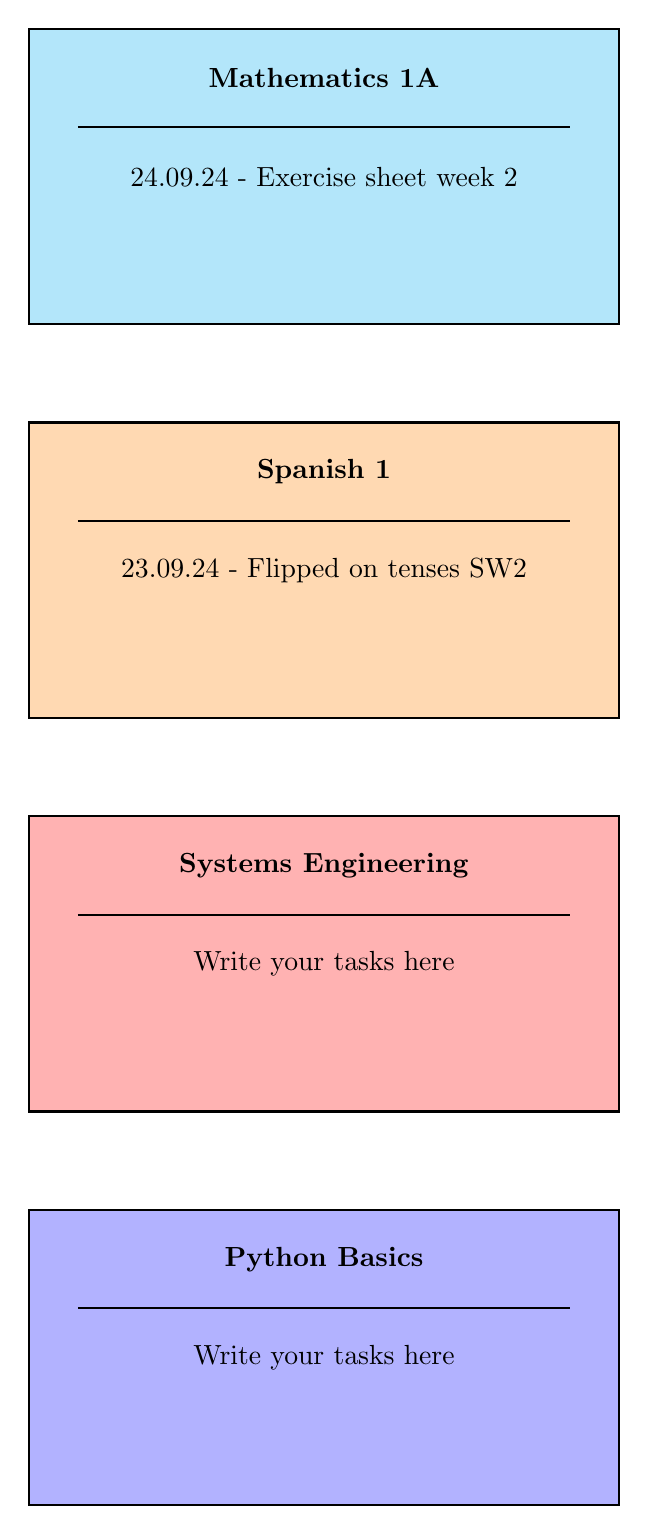
\begin{tikzpicture}[scale=1.25]
                % First subject: Mathematics 1A
                \draw[thick, fill=cyan!30] (0,0) rectangle (6,3);
                \node at (3,2.5) {\textbf{Mathematics 1A}};
                \draw[thick] (0.5, 2) -- (5.5, 2);
                \node at (3,1.5) {24.09.24 - Exercise sheet week 2};
                
                % Third subject: Spanish 1
                \draw[thick, fill=orange!30] (0,-4) rectangle (6,-1);
                \node at (3,-1.5) {\textbf{Spanish 1}};
                \draw[thick] (0.5,-2) -- (5.5,-2);
                \node at (3,-2.5) {23.09.24 - Flipped on tenses SW2};
            
                % Fifth subject: Systems Engineering
                \draw[thick, fill=red!30] (0,-8) rectangle (6,-5);
                \node at (3,-5.5) {\textbf{Systems Engineering}};
                \draw[thick] (0.5,-6) -- (5.5,-6);
                \node at (3,-6.5) {Write your tasks here};
                
                % Seventh subject: Python Basics
                \draw[thick, fill=blue!30] (0,-12) rectangle (6,-9);
                \node at (3,-9.5) {\textbf{Python Basics}};
                \draw[thick] (0.5,-10) -- (5.5,-10);
                \node at (3,-10.5) {Write your tasks here};
            \end{tikzpicture}
        \end{flushleft}
\end{wrapfigure}

\phantom{}

\vspace{-.4cm}
\begin{flushright}
    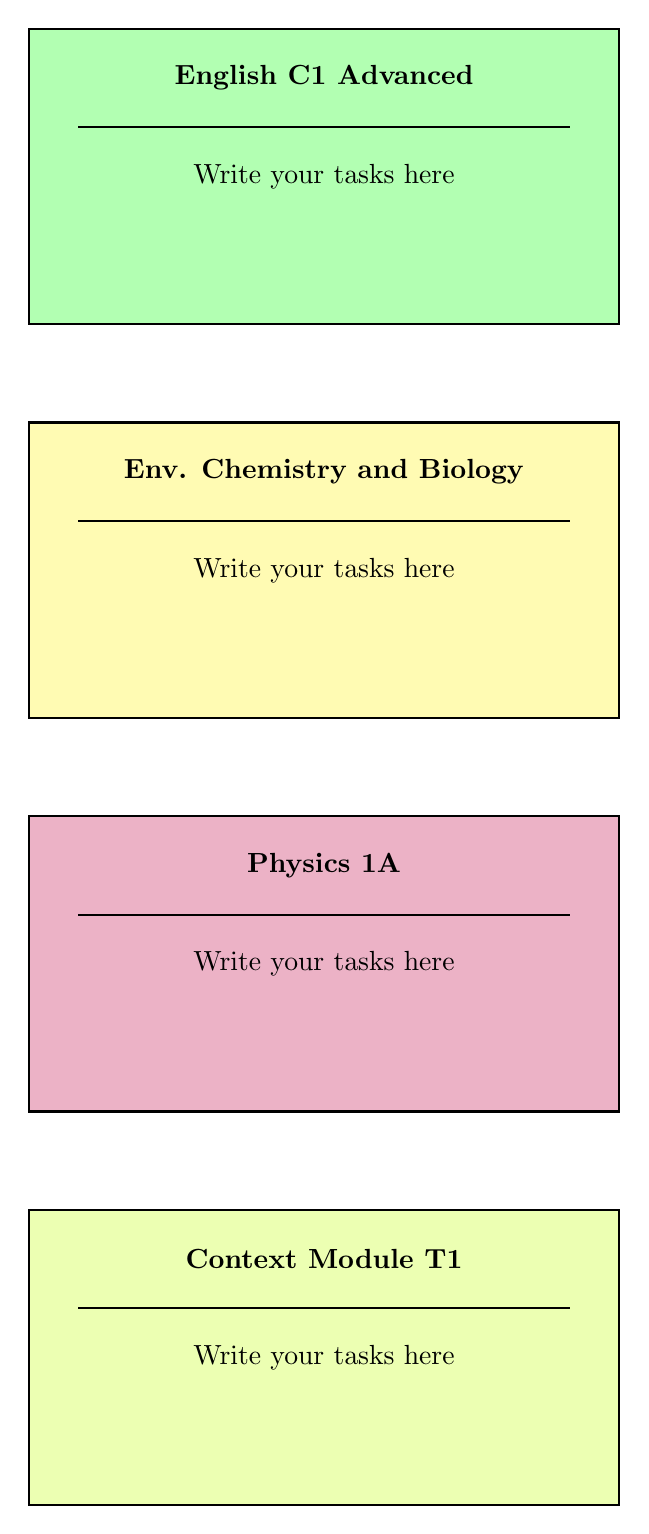
\begin{tikzpicture}[scale=1.25]
        % Second subject: English C1 Advanced
        \draw[thick, fill=green!30] (7,0) rectangle (13,3);
        \node at (10,2.5) {\textbf{English C1 Advanced}};
        % Space for tasks
        \draw[thick] (7.5, 2) -- (12.5, 2);
        \node at (10,1.5) {Write your tasks here};
        
        % Fourth subject: Environmental Chemistry and Biology
        \draw[thick, fill=yellow!30] (7,-4) rectangle (13,-1);
        \node at (10,-1.5) {\textbf{Env. Chemistry and Biology}};
        \draw[thick] (7.5,-2) -- (12.5,-2);
        \node at (10,-2.5) {Write your tasks here};
        
        % Sixth subject: Physics 1A
        \draw[thick, fill=purple!30] (7,-8) rectangle (13,-5);
        \node at (10,-5.5) {\textbf{Physics 1A}};
        \draw[thick] (7.5,-6) -- (12.5,-6);
        \node at (10,-6.5) {Write your tasks here};
        
        % Eighth subject: Context Module T1
        \draw[thick, fill=lime!30] (7,-12) rectangle (13,-9);
        \node at (10,-9.5) {\textbf{Context Module T1}};
        \draw[thick] (7.5,-10) -- (12.5,-10);
        \node at (10,-10.5) {Write your tasks here};
    \end{tikzpicture}
\end{flushright}
\wrapfill





\end{document}
